% =====================================================================
%  Mémoire de stage / d'alternance — Master Informatique
%  Thème : Réduction de la dette technique et enjeux business associés
%  Entreprises : Free Mobile & Beemo Technologie
%
%  Compilation : latexmk -pdf main.tex
%               (ou ./build.sh)
% =====================================================================
\documentclass[12pt,a4paper,oneside]{report}

% ---------- Langue & encodage ----------------------------------------
\usepackage[T1]{fontenc}
\usepackage[utf8]{inputenc}
\usepackage[french]{babel}
\usepackage{lmodern}
\usepackage{microtype}

% ---------- Mise en page ---------------------------------------------
\usepackage[a4paper,margin=2.5cm]{geometry}
\usepackage{setspace}
\onehalfspacing
\usepackage{parskip}
\sloppy                 % évite les débordements de marge
\usepackage{emptypage}  % pages blanches réellement vides

% ---------- Justification & coupures ---------------------------------
\hyphenation{re-tro-in-gé-nie-rie}

% ---------- Graphismes, couleurs, tableaux ---------------------------
\usepackage{graphicx}
\graphicspath{{figures/}}
\usepackage{xcolor}
\usepackage{booktabs}
\usepackage{array}
\usepackage{tabularx}
\usepackage{float}
\usepackage{caption}
\captionsetup{font=small,labelfont=bf}
\usepackage{pgfgantt}          % diagramme de Gantt (annexe)

% ---------- Page de couverture (maquette « Page de garde ») ----------
\usepackage{letterspace}        % \textls[...]{} : interlettrage
\usepackage{ragged2e}
\usepackage{tikz}               % cadre fin en filigrane sur la couverture
\usepackage{ebgaramond}         % serif académique — réservé à la couverture
\renewcommand*\rmdefault{lmr}   % …le corps du mémoire reste en Latin Modern
                                % (\ebgaramond bascule localement sur la garde)
\definecolor{ink}{HTML}{1A1A1A}
\definecolor{muted}{HTML}{5B5B5B}
\definecolor{coverline}{HTML}{CFCFCF}
\definecolor{coral}{HTML}{F0625F}
\definecolor{coraldeep}{HTML}{D94E4B}

% ---------- En-têtes / pieds de page ---------------------------------
\usepackage{fancyhdr}
\pagestyle{fancy}
\fancyhf{}
\fancyhead[L]{\nouppercase{\leftmark}}
\fancyhead[R]{\thepage}
\renewcommand{\headrulewidth}{0.4pt}
\fancypagestyle{plain}{\fancyhf{}\fancyfoot[C]{\thepage}\renewcommand{\headrulewidth}{0pt}}

% ---------- Code source ----------------------------------------------
\usepackage{listings}
\definecolor{codegray}{gray}{0.95}
\definecolor{codekw}{rgb}{0.13,0.29,0.53}
\definecolor{codecomment}{rgb}{0.30,0.55,0.30}
\definecolor{codestr}{rgb}{0.64,0.08,0.08}
\lstset{
  backgroundcolor=\color{codegray},
  basicstyle=\ttfamily\footnotesize,
  keywordstyle=\color{codekw}\bfseries,
  commentstyle=\color{codecomment}\itshape,
  stringstyle=\color{codestr},
  numbers=left, numberstyle=\tiny\color{gray}, numbersep=8pt,
  frame=single, rulecolor=\color{gray!40},
  breaklines=true, showstringspaces=false,
  tabsize=2, captionpos=b,
  literate={é}{{\'e}}1 {è}{{\`e}}1 {à}{{\`a}}1 {ù}{{\`u}}1 {ê}{{\^e}}1 {ç}{{\c c}}1 {â}{{\^a}}1 {î}{{\^i}}1 {ô}{{\^o}}1 {û}{{\^u}}1 {ë}{{\"e}}1 {ï}{{\"i}}1 {ü}{{\"u}}1 {É}{{\'E}}1 {È}{{\`E}}1 {À}{{\`A}}1 {œ}{{\oe}}1 {Œ}{{\OE}}1
}

% ---------- Glossaire / acronymes ------------------------------------
\usepackage[acronym,toc,nonumberlist]{glossaries}
\makeglossaries
% =====================================================================
%  Définitions du glossaire et des acronymes
%  (référencés dans le texte avec \gls{clé} ou \acrshort{clé})
% =====================================================================

% ---------- Acronymes ------------------------------------------------
\newacronym{ci}{CI}{Continuous Integration (intégration continue)}
\newacronym{cd}{CD}{Continuous Delivery / Deployment}
\newacronym{sdk}{SDK}{Software Development Kit}
\newacronym{api}{API}{Application Programming Interface}
\newacronym{abi}{ABI}{Application Binary Interface}
\newacronym{ide}{IDE}{Integrated Development Environment}
\newacronym{tdd}{TDD}{Test-Driven Development}
\newacronym{poc}{PoC}{Proof of Concept}
\newacronym{roi}{ROI}{Return On Investment (retour sur investissement)}
\newacronym{qa}{QA}{Quality Assurance (assurance qualité)}
\newacronym{vcs}{VCS}{Version Control System}
\newacronym{e2e}{E2E}{End-to-End (test de bout en bout)}

% ---------- Termes ---------------------------------------------------
\newglossaryentry{dette-technique}{
  name={dette technique},
  description={Coût implicite des retouches futures induit par le choix
  d'une solution rapide plutôt que d'une approche meilleure mais plus
  longue à mettre en œuvre. Se rembourse par le refactoring ; génère des
  « intérêts » sous forme de ralentissement du développement}
}
\newglossaryentry{test-regression}{
  name={test de non-régression},
  description={Test vérifiant qu'une modification du code n'a pas
  réintroduit de défaut ni cassé une fonctionnalité existante}
}
\newglossaryentry{test-integration}{
  name={test d'intégration},
  description={Test validant le bon fonctionnement conjoint de plusieurs
  composants assemblés, par opposition au test unitaire}
}
\newglossaryentry{fork}{
  name={fork},
  description={Divergence d'une base de code en plusieurs variantes
  maintenues en parallèle, partageant une origine commune}
}
\newglossaryentry{retro-ingenierie}{
  name={rétro-ingénierie},
  description={Analyse d'un système ou binaire existant pour en
  comprendre la structure et le comportement, en l'absence de
  documentation ou de sources complètes}
}
\newglossaryentry{toolchain}{
  name={chaîne de compilation (toolchain)},
  description={Ensemble des outils (compilateur, éditeur de liens,
  bibliothèques) permettant de transformer le code source en binaire
  exécutable pour une cible donnée}
}


% ---------- Liens hypertextes (à charger en dernier) -----------------
\usepackage[hidelinks]{hyperref}
\hypersetup{
  pdftitle={Mémoire d'alternance — Réduction de la dette technique},
  pdfauthor={Jérémy Hurel}
}

% =====================================================================
\begin{document}

% ----------------------- Page de couverture --------------------------
% =====================================================================
%  Page de couverture (page de garde)
%  Reproduit la maquette « Page de garde » : sobre, académique,
%  centrée et institutionnelle (logos UM / FdS / LIRMM, titre encadré
%  de filets, accent corail de l'UM, bloc encadrement + année).
%
%  Logos attendus dans figures/ : logo-um.png, logo-fds.png, logo-lirmm.png
%  Police EB Garamond restreinte à cette page (cf. préambule main.tex).
% =====================================================================

% ---- Petits utilitaires (locaux à la couverture) --------------------
\newcommand{\sclabel}[1]{{\footnotesize\textls[180]{\textsc{#1}}}}
\newcommand{\coralrule}{{\color{coral}\rule{38mm}{1.2pt}}}

\begin{titlepage}
\thispagestyle{empty}
\singlespacing              % composition serrée (≠ corps en interligne 1,5)
\setlength{\parskip}{0pt}
\ebgaramond                 % la garde est composée en EB Garamond
\color{ink}
\centering

% Cadre fin façon « frame inset » (filet en filigrane, à 11 mm des bords)
\begin{tikzpicture}[remember picture,overlay]
  \draw[coverline,line width=0.4pt]
    ([shift={(11mm,-11mm)}]current page.north west)
    rectangle
    ([shift={(-11mm,11mm)}]current page.south east);
\end{tikzpicture}

% ===================== EN-TÊTE : LOGOS =====================
\noindent
\begin{minipage}[c]{0.30\linewidth}\centering
  
\includegraphics[height=24mm]{logo-um.png}
\end{minipage}\hfill
\begin{minipage}[c]{0.36\linewidth}\centering
  
\includegraphics[height=15mm]{logo-fds.png}
\end{minipage}\hfill
\begin{minipage}[c]{0.30\linewidth}\centering
  
\includegraphics[height=11mm]{logo-lirmm.png}
\end{minipage}

\vspace{7mm}
{\large\textls[160]{\MakeUppercase{Université de Montpellier}}}\\[1.5mm]
{\color{muted}\textls[110]{\textsc{Faculté des Sciences — Master Informatique}}}

\vspace{5mm}
\coralrule

% ===================== BLOC CENTRAL =====================
\vfill

{\color{coraldeep}\textls[230]{\textsc{Mémoire de fin d'études}}}

\vspace{3.5mm}
{\large\textbf{Master 2 Informatique} — Parcours Génie Logiciel (GL)}

\vspace{12mm}
{\color{ink}\rule{\linewidth}{0.8pt}}\\[8mm]
{\fontsize{27}{32}\selectfont Réduction de la dette technique\\[1mm]
dans un environnement de production}\\[7mm]
{\itshape\color{muted}\large Mémoire rédigé à l'issue de deux années d'alternance}\\[8mm]
{\color{ink}\rule{\linewidth}{0.8pt}}

\vspace{11mm}
{\color{muted}\begin{minipage}{0.82\linewidth}\centering
  Travaux réalisés dans le cadre d'un contrat d'apprentissage au sein de\\
  {\color{ink}\textsc{Free Mobile}} et {\color{ink}\textsc{Beemo Technologie}}.
\end{minipage}}

\vspace{7mm}
\noindent\begin{minipage}{\linewidth}\centering
  
\includegraphics[height=13mm]{logo-free-mobile.png}\hspace{16mm}
  
\includegraphics[height=13mm]{logo-beemo.png}
\end{minipage}

\vfill

% ===================== PIED : ENCADREMENT =====================
{\color{coverline}\rule{\linewidth}{0.4pt}}\\[5mm]
\noindent
\begin{minipage}[t]{0.40\linewidth}\RaggedRight
  {\color{coraldeep}\sclabel{Présenté par}}\\[2.8mm]
  Jérémy Hurel
\end{minipage}\hfill
\begin{minipage}[t]{0.55\linewidth}\RaggedLeft
  {\color{coraldeep}\sclabel{Encadrement}}\\[2.8mm]
  David Desmarest~{\itshape\color{muted}\small— tuteur entreprise}\\[1mm]
  Mickaël Montassier~{\itshape\color{muted}\small— tuteur universitaire}
\end{minipage}

\vspace{7mm}
{\textls[260]{\MakeUppercase{Année universitaire 2024 -- 2026}}}

\end{titlepage}


% ----------------------- Pages liminaires ----------------------------
\pagenumbering{roman}

% Remerciements
\chapter*{Remerciements}
\addcontentsline{toc}{chapter}{Remerciements}

% TODO : remercier (1/2 page max)
% - l'encadrant entreprise et l'équipe chez Free Mobile
% - l'encadrant entreprise et l'équipe chez Beemo Technologie
% - l'encadrant universitaire
% - toute personne ayant contribué à l'alternance

\emph{[À rédiger — une demi-page suffit.]}


% Résumé / Abstract
\chapter*{Résumé}
\addcontentsline{toc}{chapter}{Résumé}

% TODO : 10-15 lignes synthétisant : contexte (alternance, 2 entreprises),
% fil rouge (dette technique & enjeux business), 4 tâches, résultats clés.

\emph{[Résumé à rédiger.]} Ce mémoire retrace une alternance menée au sein
de deux entreprises — Free Mobile puis Beemo Technologie — autour d'un fil
conducteur commun : la réduction de la \gls{dette-technique} et les enjeux
business qui lui sont associés. \emph{[...]}

\vspace{1em}
\noindent\textbf{Mots-clés :} dette technique, tests automatisés,
non-régression, intégration continue, rétro-ingénierie, qualité logicielle.

\vspace{2em}
\noindent\textbf{Abstract.} \emph{[Traduction anglaise du résumé —
facultatif mais apprécié.]}


% Table des matières
\cleardoublepage
\tableofcontents

% (optionnel) listes des figures / tableaux
% \listoffigures
% \listoftables

% ----------------------- Corps du mémoire ----------------------------
\cleardoublepage
\pagenumbering{arabic}

\chapter{Introduction}
\label{chap:intro}

% =====================================================================
%  Objectif (cf. INSTRUCTION) : présenter le CONTEXTE du stage (place
%  dans le cursus, entreprises, dates) et SUCCINCTEMENT le sujet.
%  Ne pas hypertrophier l'introduction : le détail technique va dans
%  les chapitres « Travaux effectués ».
% =====================================================================

\section{Contexte de l'alternance}
% TODO : place dans le cursus (Master Informatique, année), nature
% (alternance), période globale, et le fait qu'elle s'est déroulée dans
% DEUX entreprises successives : Free Mobile puis Beemo Technologie.
\emph{[À rédiger.]}

\section{Le fil conducteur : la dette technique}
% TODO : amener le thème. Idée directrice : derrière des missions
% techniques variées (framework de test, portage multi-forks,
% rétro-ingénierie de compilation, développement de feature), un même
% enjeu — maîtriser/réduire la dette technique — et un même argument
% business — vitesse de livraison, fiabilité, coût de maintenance.
\emph{[À rédiger : poser la problématique et les enjeux business.]}

\section{Problématique}
% TODO : formuler la question centrale, p.ex. :
% « Comment des actions d'ingénierie ciblées permettent-elles de réduire
%  la dette technique, et en quoi se traduisent-elles en valeur pour
%  l'entreprise ? »
\emph{[À rédiger.]}

\section{Plan du mémoire}
% TODO : annoncer brièvement le déroulé (entreprises, environnement
% technique, veille sur la dette technique, puis les 4 tâches, conclusion).
\emph{[À rédiger.]}

\chapter{Présentation des entreprises}
\label{chap:entreprises}

% =====================================================================
%  RAPPEL INSTRUCTION : cette partie ne doit EN AUCUN CAS dépasser
%  deux pages au total (les deux entreprises comprises). Rester factuel,
%  éviter le copié-collé de plaquette commerciale.
% =====================================================================

\section{Free Mobile}
Free Mobile est un opérateur de télécommunications du groupe Iliad, fondé
par Xavier Niel. L'entreprise est notamment connue pour être entrée sur le
marché de la téléphonie mobile de manière agressive, en particulier avec son
forfait à deux euros. Au-delà de ses offres commerciales, Free Mobile fait
partie des rares opérateurs à maîtriser l'ensemble de leurs logiciels en
interne : tout leur cœur de réseau y est développé, de même que la
valorisation, et l'entreprise dispose en outre d'une section R\&D dédiée à
ses propres équipements matériels.

J'ai intégré l'équipe Valo, rattachée au Core SI. Cette équipe a la charge
du logiciel de valorisation, qui calcule en temps réel la valeur de l'ensemble des appels
passés en téléphonie mobile sur les différents réseaux.

À mon arrivée, ce logiciel se trouvait dans un contexte de dette technique
élevée : l'ingénieur qui en assurait la maintenance avait quitté
l'entreprise, et plusieurs règles de génie logiciel n'avaient pas été
respectées : une partie des sources, par exemple, n'était pas versionnée. L'équipe, montée et dirigée par David Desmarest, s'est vu confier une
mission de reprise de contrôle de ce logiciel.

Mon rôle y était transverse au travail de l'équipe de développement :
supporter celle-ci en produisant des outils internes, au premier rang
desquels le framework de test détaillé à la section~\ref{chap:t3}.

\section{Beemo Technologie}
Beemo Technologie est une entreprise d'une vingtaine d'années spécialisée
dans la sauvegarde de données. Sa particularité est de ne pas se limiter à
un logiciel installé sur une machine du client, mais de proposer une
solution clé en main : des boîtiers (\emph{box}) déployés au sein de
l'entreprise, voire chez son dirigeant, qui assurent la sauvegarde et la
duplication des données, et donc leur redondance en cas de perte.
Une partie de la solution est également déployée dans le cloud, afin de renforcer cette redondance.

L'entreprise compte une trentaine d'employés et dispose de clients et de
partenaires principalement en France, et s'étend à d'autres pays européens et
africains ; son développement actuel porte sur le continent africain. Une partie des effectifs est dédiée à une \emph{hotline},
reconnue pour sa réactivité et son efficacité dans la résolution des
problèmes. Beemo se distingue enfin par le caractère souverain de sa solution
de sauvegarde, un atout particulièrement recherché dans le contexte actuel.

Mon arrivée chez Beemo a fait suite à une proposition de David Desmarest, qui,
après avoir quitté Free Mobile, y avait pris le \emph{lead} de l'équipe de
développement. Ma décision de le
suivre a répondu à plusieurs facteurs. L'équipe que je quittais traversait une
restructuration qui faisait peser une incertitude sur son devenir, sur laquelle
le management communiquait peu ; je m'y retrouvais paradoxalement parmi les
développeurs les plus anciens, la plupart d'entre eux ayant rejoint l'équipe
après moi. L'orientation méthodologique impulsée par la direction privilégiait
en outre des correctifs rapides, une manière d'aborder la dette technique qui
correspondait moins à la mienne. La proposition de David offrait à l'inverse un
projet dont je connaissais la direction et les perspectives, lui aussi centré
sur la réduction de la dette technique, et la possibilité de revenir à terme au
développement C++ : une perspective qui avait compté dans mon choix initial et
que la situation ne garantissait plus.

À la différence de Free Mobile, où mon rôle était transverse et orienté support,
j'occupais désormais un poste de développeur travaillant directement sur le
fonctionnel. Le contexte restait toutefois marqué par la dette technique :
l'enjeu était de demeurer productif face au marché, c'est-à-dire de
continuer à livrer de nouvelles fonctionnalités, tout en résorbant
progressivement cette dette.

\section{Positionnement des missions}
Sept missions jalonnent ces deux années : cinq chez Free Mobile, deux chez
Beemo Technologie, ces dernières étant encore en cours au moment de la
rédaction. Plutôt que de les présenter dans l'ordre chronologique, restitué
par le diagramme de Gantt en annexe~\ref{chap:annexes}, ce mémoire les
regroupe par nature, en trois chapitres thématiques : \textbf{outiller la productivité et
standardiser l'environnement de développement}, \textbf{rendre testable un
logiciel legacy} pour résorber les régressions et s'en prémunir, et
\textbf{développer du code à visée de production dans un existant endetté}.
Le tableau~\ref{tab:missions} en donne la vue d'ensemble.

\begin{table}[H]
\centering
\begin{tabularx}{\textwidth}{@{}l l X@{}}
\toprule
\textbf{Thème / Entreprise} & \textbf{Mission} & \textbf{Objectif au regard de la dette technique} \\
\midrule
\multicolumn{3}{@{}l}{\emph{Outils : productivité et standardisation de l'environnement de développement}} \\
Free Mobile & Duplication Grafana & Fiabiliser la réplication de la supervision \\
Free Mobile & Compilation C++ & Maîtriser le coût de compilation (CPU/RAM) \\
Beemo      & Rétro-ing. SDK    & Débloquer et documenter une compilation existante \\
\midrule
\multicolumn{3}{@{}l}{\emph{Testabilité d'un logiciel legacy}} \\
Free Mobile & Framework de test & Industrialiser la non-régression \\
Free Mobile & Extension VS Code & Ouvrir l'usage du framework à toute l'équipe \\
Free Mobile & Portage multi-forks & Mutualiser la qualité sur les variantes \\
\midrule
\multicolumn{3}{@{}l}{\emph{Code à visée de production dans un existant endetté}} \\
Beemo      & Immuabilité       & Livrer une fonctionnalité sans accroître la dette \\
\bottomrule
\end{tabularx}
\caption{Vue d'ensemble des missions, regroupées par nature.}
\label{tab:missions}
\end{table}

\chapter{Environnement technique}
\label{chap:env}

% =====================================================================
%  RAPPEL INSTRUCTION : présenter SUCCINCTEMENT les technologies, outils,
%  méthodes. Éviter l'inventaire lassant : ne lister que ce qui est
%  réellement mobilisé dans les tâches, et regrouper par thème.
% =====================================================================

\section{Langages et bibliothèques}
% TODO : langages utilisés (ex. Python/C/C++/Shell...), frameworks de test
% (ex. pytest, ...), bibliothèques clés. Une phrase de justification par item.
\emph{[À rédiger.]}

\section{Outils de build et de compilation}
% TODO : chaîne de compilation, SDK, gestionnaires de dépendances,
% (utile en amont de la tâche 3 « rétro-ingénierie »).
\emph{[À rédiger.]}

\section{Gestion de version et intégration continue}
% TODO : \gls{vcs} (Git ?), forge (GitLab/GitHub ?), pipelines \gls{ci}/\gls{cd}.
\emph{[À rédiger.]}

\section{Méthodologie et gestion de projet}
% TODO : méthode (agile/scrum/kanban ?), outils de ticketing, rituels.
\emph{[À rédiger.]}

\chapter{Appropriation scientifique : la dette technique et ses enjeux business}
\label{chap:veille}

% =====================================================================
%  Ce chapitre + « Travaux effectués » doivent représenter AU MOINS la
%  moitié du mémoire. C'est ici qu'on pose le cadre conceptuel qui sert
%  de grille de lecture aux 4 tâches. Mobiliser la bibliographie
%  (references.bib) : Cunningham, Fowler, Feathers, Kruchten, Humble.
% =====================================================================

\section{Définition et métaphore}
% TODO : la métaphore de Cunningham (1992) \cite{cunningham1992} ;
% « principal » vs « intérêts » ; pourquoi la dette n'est pas toujours
% une mauvaise chose (dette délibérée vs accidentelle).
\emph{[À rédiger.]}

\section{Typologie de la dette technique}
% TODO : dette de code, de test, d'architecture, de documentation,
% de dépendances/build. Quadrant de Fowler (délibérée/imprudente...).
% Relier chaque type aux tâches du mémoire.
\emph{[À rédiger.]}

\section{Enjeux business}
% TODO : le cœur du thème. Traduire la dette en termes d'entreprise :
% - vélocité de livraison et time-to-market
% - coût de maintenance et risque de régression
% - fiabilité / image (surtout pour un opérateur télécom)
% - \gls{roi} d'un investissement dans les tests / l'outillage
\emph{[À rédiger.]}

\section{Leviers de réduction}
% TODO : tests automatisés & non-régression, \gls{ci}/\gls{cd},
% refactoring \cite{fowler2018}, maîtrise du legacy \cite{feathers2004},
% documentation/outillage. Annoncer comment chaque tâche actionne un levier.
\emph{[À rédiger.]}

\section{Grille de lecture des missions}
% TODO : petit paragraphe-charnière reliant la théorie aux 4 tâches qui
% suivent (tableau optionnel : tâche -> type de dette -> levier -> bénéfice).
\emph{[À rédiger.]}


% --- Travaux effectués : tâches regroupées par NATURE (cf. INSTRUCTION),
%     la chronologie exacte étant donnée par le Gantt en annexe. ---------
% Volet 1 — Outiller la qualité : supervision et non-régression
\chapter{Tâche 1 — Outil de duplication de configuration Grafana}
\label{chap:t1}
% Entreprise : Free Mobile

% =====================================================================
%  Trame conseillée (réutilisée pour chaque tâche) :
%  1. Contexte & dette technique de départ
%  2. Objectif de la mission
%  3. Conception / choix techniques
%  4. Réalisation (extraits de code COMMENTÉS, schémas — PAS de code entier)
%  5. Difficultés rencontrées
%  6. Résultats & bénéfice business (réduction de la dette)
% =====================================================================

\section{Contexte et dette technique initiale}
La supervision de la valorisation s'appuie sur \textbf{Grafana}, qui agrège dans
des \emph{dashboards} les métriques remontées par le \emph{Valo Engine}. Or cette
supervision n'existe pas sur une seule instance : on en retrouve plusieurs
— typiquement une par environnement (développement, recette, production) ou par
réseau — qui doivent présenter les \textbf{mêmes tableaux de bord}. Faire vivre
ces instances en parallèle suppose donc de \textbf{répliquer} la configuration de
l'une vers les autres à chaque évolution.

Cette réplication ne se résume pas à une copie : chaque tableau de bord référence
ses \textbf{sources de données} (\emph{datasources}) par un \textbf{identifiant
propre à l'instance}. Le même tableau, copié tel quel d'une instance à l'autre,
pointe alors vers des identifiants qui n'y existent pas, et l'affichage se
retrouve cassé. La synchronisation manuelle — export, copie, puis correction au
cas par cas des identifiants — était donc à la fois \textbf{fastidieuse et source
d'erreurs} : une dette d'outillage sur la chaîne de supervision elle-même.

\section{Objectif de la mission}
La mission consistait à \textbf{reprendre le travail d'un stagiaire}, qui avait
amorcé un \gls{poc} sur ce sujet, pour en faire un outil exploitable. Le but :
\textbf{dupliquer l'ensemble des tableaux de bord} d'une instance Grafana vers une
autre, puis \textbf{réécrire automatiquement} les identifiants de sources de
données pour qu'ils correspondent à ceux de l'instance cible. Le cœur du problème
est donc un \textbf{appariement} : faire correspondre, deux à deux, les sources
de données de l'instance d'origine et celles de l'instance de destination, afin
de substituer chaque identifiant par son équivalent.

\section{Conception et choix techniques}
La logique métier est directe : Grafana expose une \gls{api} HTTP permettant de
\textbf{lister} les tableaux de bord et les sources de données d'une instance,
puis d'y \textbf{créer} de nouveaux objets. L'outil interroge l'instance source,
construit une \textbf{table de correspondance} entre les sources de données des
deux instances (appariées par nom), puis parcourt chaque tableau de bord pour y
\textbf{remplacer} les identifiants avant de le pousser sur l'instance cible.

L'enjeu de conception portait surtout sur l'\textbf{interface}. Plutôt qu'une
ligne de commande aride, l'outil a été doté d'une \textbf{interface en mode texte}
(\gls{tui}) à l'aide du framework Python \textbf{Textual}. Ce framework a été une
\textbf{découverte marquante} : il permet de décrire une interface terminal selon
un modèle très proche du développement web — une structure de composants
apparentée au \emph{HTML}, mise en forme par des feuilles de style apparentées au
\emph{CSS}. On obtient ainsi, dans un simple terminal, une interface interactive
(listes, sélection des instances, validation de l'appariement) sans quitter
l'environnement de travail des administrateurs.

\section{Réalisation}
% TODO : remplacer par un extrait réel du dépôt (illustratif, pas le code entier).
Le cœur de l'outil tient dans la réécriture des identifiants : à partir de la
table de correspondance construite entre les deux instances, chaque référence à
une source de données présente dans un tableau de bord est substituée par son
équivalent côté cible.

\begin{lstlisting}[language=Python,caption={Réécriture des identifiants de sources de données lors de la duplication (extrait illustratif).},label={lst:t1}]
# correspondance : datasource de l'instance source -> datasource de la cible,
# appariées par leur nom (ex. "prometheus-valo" présent sur les deux instances)
correspondance = apparier_par_nom(sources_origine, sources_cible)

def reecrire(dashboard):
    # on substitue chaque identifiant de datasource par son équivalent cible ;
    # un dashboard copié sans cette étape pointerait vers des IDs inexistants
    for panel in dashboard["panels"]:
        ancien = panel["datasource"]["uid"]
        panel["datasource"]["uid"] = correspondance[ancien]
    return dashboard
\end{lstlisting}

\section{Difficultés rencontrées}
S'agissant de ma \textbf{première tâche} dans l'équipe, l'enjeu principal n'était
pas tant la complexité — le besoin était circonscrit et la mission relativement
\textbf{rapide} — que la \textbf{prise en main} de l'environnement : le mode de
travail de l'équipe, le dépôt, et la reprise d'un \gls{poc} déjà entamé par un
tiers. La principale subtilité technique tenait à la \textbf{robustesse de
l'appariement} des sources de données, l'appariement par nom supposant une
nomenclature cohérente d'une instance à l'autre.

\section{Résultats et bénéfice business}
% TODO : quantifier si possible (temps de synchronisation avant/après, erreurs
%        évitées). Relier au thème dette technique (chap.~\ref{chap:veille}).
L'outil a transformé une synchronisation manuelle et faillible en une opération
\textbf{automatisée et reproductible}, supprimant la classe d'erreurs liée aux
identifiants de sources de données mal réécrits. Au-delà du livrable, cette
première mission a joué un rôle de \textbf{mise en jambe} : prise de contact avec
l'équipe et son environnement, et découverte de Textual, un framework réinvesti
par la suite. \emph{[À compléter : gain de temps mesuré sur la synchronisation
des instances.]}

\chapter{Tâche 3 — Framework de test d'intégration et de non-régression}
\label{chap:t3}
% Entreprise : Free Mobile

% =====================================================================
%  Trame conseillée (réutilisée pour chaque tâche) :
%  1. Contexte & dette technique de départ
%  2. Objectif de la mission
%  3. Conception / choix techniques
%  4. Réalisation (extraits de code COMMENTÉS, schémas — PAS de code entier)
%  5. Difficultés rencontrées
%  6. Résultats & bénéfice business (réduction de la dette)
% =====================================================================

\section{Contexte et dette technique initiale}
% TODO : avant ton arrivée, comment la non-régression était-elle gérée ?
% (tests manuels ? absence de filet de sécurité ? régressions récurrentes ?)
% Quantifier si possible le « coût » de cette dette.
La non-régression du \emph{Valo Engine} reposait initialement sur une suite de
tests écrits en Lua. Ce langage permettait de scripter des scénarios, mais ne
s'avérait pas le mieux adapté à ce que l'on cherchait à faire. Sa nature
\textbf{impérative} laissait en effet au rédacteur d'un test toute latitude pour
y introduire de la logique : un test pouvait dès lors échouer non à cause d'une
régression du logiciel testé, mais à cause d'un défaut du test lui-même. La
frontière entre code de test et code testé devenait floue, ce qui fragilisait la
confiance accordée à ce filet de sécurité. À cela s'ajoutait un couplage de bas
niveau : le protocole de communication du moteur — un protocole TCP décrit en C
— était embarqué dans le Lua, ce qui rendait la suite délicate à maintenir.

\section{Objectif de la mission}
% TODO : concevoir un framework de tests d'intégration / non-régression /
% fonctionnels pour le programme initial.
L'objectif était de remplacer cette suite Lua par un framework dédié, reposant
sur des scénarios \textbf{déclaratifs}, volontairement plus contraignants. En
restreignant fortement la forme des tests — un scénario décrit \emph{quoi}
vérifier, jamais \emph{comment} —, on garantit que l'échec d'un test, dès lors
que le framework se trouve dans une version stable, provient bien du code du
logiciel testé et non de la mécanique de test. Le nouveau framework devait au
minimum couvrir le périmètre fonctionnel déjà assuré par le Lua : la simulation
des trames d'appel (appels voix, envoi de SMS et de MMS, consommation de data)
ainsi que la vérification des données ainsi produites.

\section{Conception et choix techniques}
% TODO : architecture du framework (runner, fixtures, jeux de données,
% rapports), langage/outils retenus et pourquoi, intégration au pipeline.

La première étape a consisté à \textbf{porter en Python} le protocole TCP par
lequel le framework dialogue avec le \emph{Valo Engine}, jusque-là décrit en C
et embarqué dans le Lua. Le module \texttt{ctypes} de Python permet de définir
des structures dont la disposition binaire est strictement équivalente à celle
de leurs homologues C ; on reconstitue ainsi un échange de trames identique à
celui du moteur sans recourir au langage natif.

Le framework prend en entrée des scénarios de test rédigés en YAML. Ces
scénarios sont analysés par un \textbf{parseur SAX}, qui présente deux
avantages : il permet de récupérer la position (ligne) de chaque instruction
— information transmise au débogueur pour offrir une exécution \emph{pas à
pas} — et il interrompt l'analyse dès la première erreur de syntaxe en
indiquant sa localisation et sa nature (arguments mal formés ou instruction
non supportée).

L'exécution repose sur une \textbf{boucle séquentielle} simple : les
instructions sont jouées les unes après les autres, sans branchement ni
retour arrière. Chaque ligne de texte est transformée en objet
\emph{instruction} suivant le patron \emph{Command} : une \emph{factory}
instancie la commande correspondante à partir d'un \emph{registry} où sont
enregistrées toutes les commandes supportées.

Autour de cette boucle, le framework fournit les services nécessaires pour
\textbf{moquer} les briques avec lesquelles le logiciel testé — le
\emph{Valo Engine} — interagit : un service simulant les équipements qui
interrogent le moteur (autorisation d'appel ou de SMS, vérification du crédit
selon la localisation) et un service recevant les notifications de seuil
émises par le moteur (courriels et messages). Enfin, un ensemble
d'instructions de \textbf{vérification} contrôle, pour une trame d'appel
donnée, la cohérence des données générées en base.

Le mécanisme de vérification reprend le principe de \emph{snapshot} déjà employé
côté Lua : les actions jouées ainsi que l'état final de la base de données sont
sérialisés, puis comparés à une trace de référence enregistrée lors d'une
exécution validée ; toute divergence signale une régression. Pour disposer
d'emblée d'une restitution des résultats exploitable — comptes rendus,
agrégation des échecs, comparable à celle d'une suite de tests classique — le
framework a été bâti comme une \textbf{surcouche de Pytest}, la génération et la
comparaison des snapshots étant déléguées à la bibliothèque \textbf{syrupy}.

\begin{figure}[H]\centering
  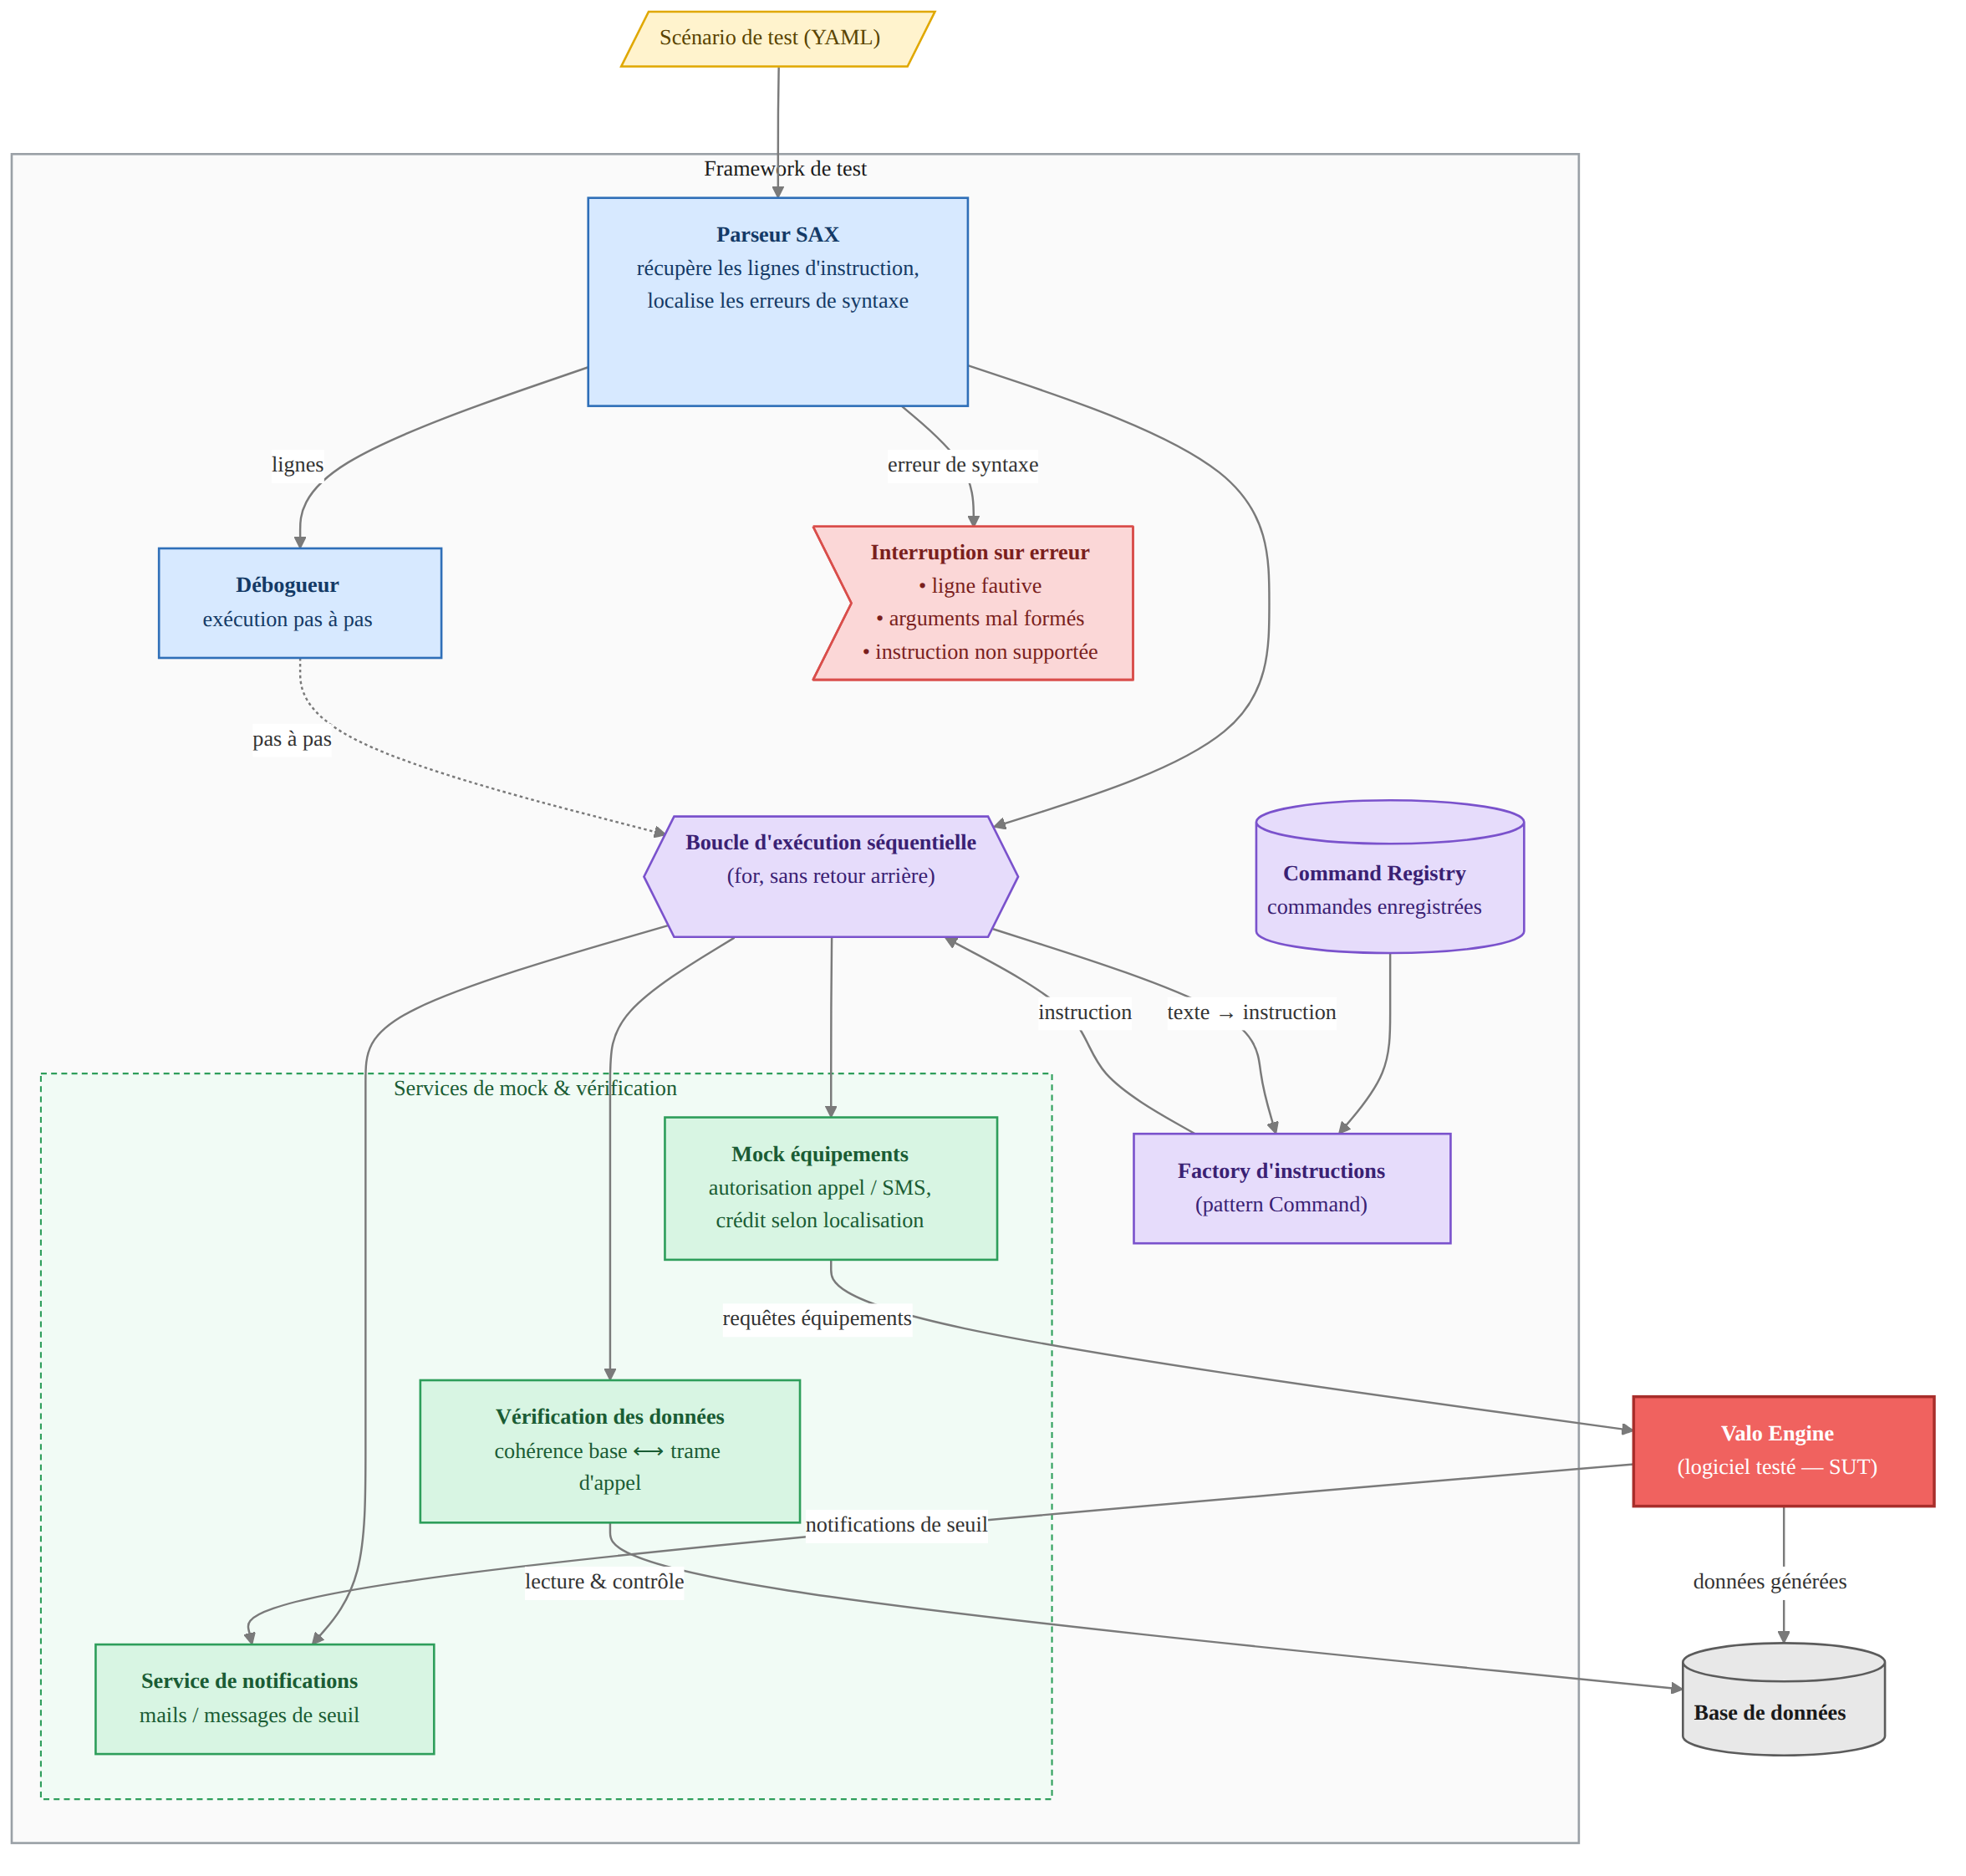
\includegraphics[width=\textwidth]{framework.png}
  \caption{Architecture du framework de test.}\label{fig:archi-t3}
\end{figure}

\section{Réalisation}
% TODO : illustrer par un EXTRAIT de code commenté (pas le code entier).
% Exemple de gabarit listing :
% \begin{lstlisting}[language=Python,caption={Définition d'un cas de test.},label={lst:t1}]
% def test_exemple():
%     ...
% \end{lstlisting}
\emph{[À rédiger.]}

\section{Difficultés rencontrées}
% TODO : ex. environnements non reproductibles, données de test, flakiness.
S'agissant de l'une des premières missions d'envergure qui m'étaient confiées,
la principale difficulté a tenu au \textbf{découpage du travail}. Plutôt que de
procéder par versions intermédiaires, livrables et vérifiables au fur et à
mesure, je me suis engagé d'emblée dans la conception complète d'une première
version couvrant l'ensemble des fonctionnalités du Lua. Ce choix a allongé le
délai avant d'obtenir un premier retour concret et m'a privé des points de
contrôle qu'un découpage plus fin aurait offerts.

Le second point, apparu avec le recul, concerne le choix de bâtir le framework
sur Pytest. Si cet outil fournit gratuitement un socle d'exécution et de
reporting éprouvé, il recèle aussi de nombreux mécanismes implicites — sa
« \emph{black magic} » — dont le comportement peut se révéler déroutant et
compliquer le développement d'une surcouche.

\section{Résultats et bénéfice business}
% TODO : couverture obtenue, régressions détectées, temps gagné,
% confiance dans les livraisons. Relier au chapitre \ref{chap:veille}.
\emph{[À rédiger.]}

\chapter{Tâche 4 — Outillage du framework : extension VS Code (LSP et débogueur)}
\label{chap:t4}
% Entreprise : Free Mobile

% =====================================================================
%  Trame conseillée (réutilisée pour chaque tâche) :
%  1. Contexte & dette technique de départ
%  2. Objectif de la mission
%  3. Conception / choix techniques
%  4. Réalisation (extraits de code COMMENTÉS, schémas — PAS de code entier)
%  5. Difficultés rencontrées
%  6. Résultats & bénéfice business (réduction de la dette)
% =====================================================================

\section{Contexte et dette technique initiale}
Une fois le framework de test livré (tâche~3, chapitre~\ref{chap:t3}), un nouveau
frein est apparu : la rédaction des tests elle-même. Les scénarios sont décrits
en YAML, support sur lequel l'écriture ne bénéficie d'aucune assistance
contextuelle. Là où des langages comme Python, Lua ou C++ disposent d'un serveur
de langage (\gls{lsp}) offrant autocomplétion et analyse syntaxique au fil de la
frappe, le YAML n'est outillé que pour la validation de schémas. Il ne propose
pas d'assistance qui tienne compte du contexte — capable, par exemple, de savoir
si l'on est en train de saisir une instruction ou l'un de ses arguments.

Or le format de test n'est pas un simple document de configuration : c'est en
réalité un langage à part entière, bâti au-dessus du YAML. On y manipule des
\textbf{instructions} — équivalentes à des fonctions —, des \textbf{constantes}
ainsi que des \textbf{variables} qui constituent les arguments passés à ces
instructions. Faute d'outillage tenant compte de cette grammaire, les erreurs de
syntaxe n'étaient découvertes qu'à l'exécution et aucun moyen n'existait
d'observer pas à pas le déroulé d'un scénario. Cette friction freinait l'adoption
du framework par l'équipe : une dette « d'outillage ».

\section{Objectif de la mission}
La mission a consisté à développer une extension \emph{Visual Studio Code},
écrite en \textbf{TypeScript}, au service du framework de la tâche~3. Cette
extension réunit deux facettes complémentaires :
\begin{itemize}
  \item un \textbf{serveur de langage} (\gls{lsp}) apportant autocomplétion,
        diagnostics en temps réel et aide à la saisie. En s'appuyant sur la
        grammaire du format de test — instructions, constantes et variables —,
        il fournit une assistance \emph{contextuelle} : il sait distinguer
        l'endroit où l'on attend une instruction de celui où l'on saisit un
        argument, et propose les complétions correspondantes ;
  \item un \textbf{débogueur} permettant d'exécuter un test puis, lorsqu'une
        instruction échoue, d'inspecter l'état du \emph{Valo Engine} au moment
        précis de l'échec, ou de progresser \emph{pas à pas} pour comprendre le
        comportement interne du moteur en fonction des trames envoyées par le
        test.
\end{itemize}

Une fonctionnalité particulièrement utile en a découlé : la possibilité de lancer
le \emph{Valo Engine} en \textbf{mode débogage} et de progresser pas à pas
\emph{à l'intérieur même de son code C++}, tout en rejouant un scénario d'appel
(\emph{call flow}) étape par étape. Le diagnostic ne se limite ainsi plus au
test, mais descend jusqu'au code natif du logiciel sous test.

\section{Conception et choix techniques}
% TODO : un SCHÉMA d'architecture serait le bienvenu :
% \begin{figure}[H]\centering
%   \includegraphics[width=0.85\textwidth]{archi-extensions-vscode.png}
%   \caption{Architecture de l'extension et son dialogue avec le framework.}
%   \label{fig:archi-t2}
% \end{figure}
Le choix du \gls{lsp} répond à un principe de \textbf{découplage} entre l'éditeur
et le langage : la logique d'analyse et de complétion est portée par un serveur
indépendant, réutilisable au-delà de VS Code par tout éditeur compatible. Le
serveur exploite la grammaire du format de test — celle-là même qu'analyse le
parseur du framework (chapitre~\ref{chap:t3}) — pour produire des complétions et
des diagnostics cohérents avec ce que le framework acceptera réellement à
l'exécution.

Le débogueur, lui, repose sur le \textbf{Debug Adapter Protocol} (\gls{dap}),
protocole standardisé par VS Code pour piloter une session de débogage au moyen
d'échanges \emph{JSON-RPC}. Côté framework, son intégration s'appuie sur un
module qui contrôle le flot d'exécution du test — mise en pause, reprise,
progression pas à pas — tout en remontant à l'éditeur les données nécessaires au
diagnostic.

Les seules données internes au framework de test ne suffisent toutefois pas à
diagnostiquer l'ensemble des problèmes : il faut aussi connaître l'état interne
du moteur. Un \textbf{service} dédié — développé par David — a donc été mis en
place pour exposer l'état des variables internes du \emph{Valo Engine}.
L'extension dialogue avec ce service via \textbf{HTTP} et restitue ces valeurs
directement dans l'\gls{ide}, aux côtés de l'état du test.

\section{Réalisation}
% TODO : remplacer les extraits ci-dessous par des extraits réels du dépôt.
%        Ils sont fournis à titre ILLUSTRATIF (pas le code entier).
Côté \gls{lsp}, le serveur s'abonne aux requêtes de complétion émises par
l'éditeur. À partir de la position du curseur, il détermine le contexte
grammatical courant et renvoie la liste des propositions adaptées — instructions
disponibles ou variables déjà déclarées.

\begin{lstlisting}[language=Java,caption={Fourniture d'autocomplétion contextuelle via le LSP (extrait illustratif, TypeScript).},label={lst:t4-lsp}]
// Déclenché par l'éditeur à chaque demande de complétion
connection.onCompletion((params) => {
  // On déduit le contexte grammatical à partir de la position du curseur
  const contexte = analyserContexte(document, params.position);

  // Selon que l'on attend une instruction ou un argument,
  // on ne propose pas le même jeu de complétions
  return contexte === "instruction"
    ? instructionsSupportees()   // liste tirée du registry du framework
    : variablesDeclarees(document);
});
\end{lstlisting}

Côté débogueur, l'adaptateur \gls{dap} traduit les ordres de l'éditeur (poser un
point d'arrêt, exécuter l'instruction suivante) en commandes pilotant le flot
d'exécution du test, puis renvoie l'état courant — instruction en cours, état du
\emph{Valo Engine} obtenu via le service HTTP.

\begin{lstlisting}[language=Java,caption={Pas à pas : pose des points d'arrêt côté adaptateur de débogage (extrait illustratif, TypeScript).},label={lst:t4-dap}]
// Requête DAP : l'éditeur transmet les lignes où s'arrêter
protocol.onSetBreakpoints((args) => {
  // Les lignes proviennent du parseur du framework,
  // qui associe chaque instruction à sa position dans le YAML
  moteurDeTest.armerPointsArret(args.lines);

  // On confirme à l'éditeur les points d'arrêt effectivement posés
  return { breakpoints: args.lines.map(verifierLigne) };
});
\end{lstlisting}

\section{Difficultés rencontrées}
La première difficulté a tenu à la \textbf{documentation de l'API d'extension de
VS Code}. Si des exemples d'extensions existent, l'\gls{api} elle-même reste
inégalement documentée, et aucun standard ne s'impose réellement quant à la
manière de structurer le code. Les exemples disponibles sont fréquemment
\textbf{monolithiques}, ce qui offre peu de modèles d'architecture réutilisables
et a imposé un travail d'expérimentation pour aboutir à une organisation
maintenable.

La seconde difficulté a porté sur l'\textbf{intégration du \gls{dap}} au
framework de test. Il a fallu adapter le protocole — fondé sur des échanges
\emph{JSON-RPC} — à un module capable de contrôler le flot d'exécution d'un test
tout en remontant les données utiles au diagnostic. La restitution de l'état
interne du moteur, obtenue par un service HTTP distinct, a par ailleurs supposé
de coordonner deux canaux de communication (\gls{dap} et HTTP) au sein d'une même
session de débogage.

\section{Résultats et bénéfice business}
% TODO : quantifier si possible (temps d'écriture d'un test, erreurs évitées,
%        taux d'adoption). Relier au thème dette technique (chap.~\ref{chap:veille}).
\emph{[À rédiger : temps d'écriture d'un test réduit grâce à l'autocomplétion et
aux diagnostics en temps réel, erreurs de syntaxe détectées avant l'exécution,
diagnostic accéléré des comportements inattendus — jusque dans le code C++ du
moteur — et, in fine, meilleure adoption du framework par l'équipe. À relier au
thème de la dette technique, chapitre~\ref{chap:veille}.]}

\chapter{Tâche 5 — Portage du framework vers les forks legacy du Valo Engine}
\label{chap:t5}
% Entreprise : Free Mobile

\section{Contexte et dette technique initiale}
% TODO : pourquoi plusieurs \gls{fork} du programme initial existent-ils ?
% Quelle dette cela crée-t-il (duplication de tests, divergence, double
% maintenance) ? C'est le « problème business » à résoudre.
Le framework de test (tâche~3, chapitre~\ref{chap:t3}) avait été conçu pour le
\emph{Valo Engine} du \textbf{réseau prépayé} de Free Mobile, un réseau alors
nouveau. Une fois ce dernier mis en production et jugé \textbf{stable}, la
stratégie de gestion de la dette technique a été révisée — une inflexion qui a
coïncidé avec le départ de David.

La stratégie initiale faisait du prépayé le socle d'une \textbf{base de code
commune et moderne}, destinée à être réutilisée par les moteurs de valorisation
des différents réseaux : on aurait ainsi migré progressivement chaque réseau
vers cette version moderne. Elle a cédé la place à une approche de \textbf{quick
fix} — que l'on pourrait presque qualifier de \emph{quick converting} —, visant
à \textbf{stabiliser au maximum} les réseaux existants sans en moderniser le
code ; la modernisation n'interviendrait, le cas échéant, qu'une fois cette
stabilisation acquise.

Or ces réseaux reposent sur autant de \gls{fork} \emph{legacy} du moteur, chacun
doté de ses spécificités métier. Plusieurs inconnues pesaient sur les
exécutables réellement en production : certains binaires n'avaient pas été mis à
jour depuis longtemps, et les sources se répartissaient entre le dépôt GitLab et
diverses machines. Toucher à ce code sans filet était d'autant plus risqué que
le \emph{Valo Engine} calcule le \textbf{coût de chaque appel} : une régression
ou une panne sur ce maillon peut engendrer des pertes \textbf{de l'ordre du
million d'euros en une semaine}. La dette tenait donc à l'absence de tout moyen
de garantir qu'un correctif n'introduise pas, par inadvertance, un
\textbf{changement de logique métier} sur l'un de ces forks.

\section{Objectif de la mission}
% TODO : faire évoluer le framework (tâche 3) pour qu'il supporte
% plusieurs forks avec un socle de tests mutualisé.
La mission a consisté à \textbf{porter le framework de test} vers l'ensemble des
forks legacy du \emph{Valo Engine}, afin de doter chaque réseau d'un filet de
non-régression \emph{avant} d'y appliquer le moindre correctif. Le périmètre
couvrait six variantes : la France \textbf{B2C} et \textbf{B2B}, les
\textbf{Caraïbes}, l'Italie \textbf{B2C} et \textbf{B2B}, ainsi que le
\textbf{proxy} italien.

L'objectif premier n'était pas de couvrir fonctionnellement chaque réseau dans
les moindres détails, mais de disposer d'un \textbf{contrôle sur le code métier}
de chaque fork : pouvoir y appliquer des correctifs avec l'assurance que la
logique de valorisation demeurait inchangée.

\section{Conception : factorisation et paramétrage}
% TODO : stratégie de portage (abstraction des différences entre forks,
% configuration par fork, tests communs vs spécifiques). Schéma avant/après.
La principale difficulté de conception tenait à l'hétérogénéité des réseaux,
qui se répartissent en deux modèles de facturation. Les réseaux en
\gls{online-charging} fonctionnent comme le prépayé : les trames d'appel, de
SMS et de data sont échangées en temps réel via un protocole TCP interne. Les
réseaux en \gls{offline-charging}, eux, ne dialoguent pas en direct avec le
moteur : celui-ci \textbf{consomme des \gls{cdr}}, c'est-à-dire des fichiers
décrivant a posteriori la consommation. Un premier chantier a donc consisté à
doter le framework de la capacité à \textbf{produire et lire des CDR} pour
simuler les équipements en \emph{offline charging}, là où il ne savait jusque-là
qu'émettre des trames TCP.

Pour absorber cette diversité, David avait amorcé une refonte du framework
articulée autour de deux notions complémentaires :
\begin{itemize}
  \item un \textbf{core} — le socle commun à toutes les versions supportées. Il
        porte la mécanique invariante : la boucle d'exécution et le
        \emph{parsing} des instructions du langage de test ;
  \item des \textbf{specs} — une par fork — qui spécifient \emph{quelles}
        instructions sont disponibles et \emph{comment} elles s'exécutent, en
        fournissant leur \textbf{implémentation runtime} propre au réseau visé.
\end{itemize}
Cette séparation \emph{core} / \emph{spec} permet de mutualiser tout ce qui ne
dépend pas du réseau et de n'isoler, fork par fork, que les différences de
comportement métier — préparant du même coup la modernisation ultérieure.

\section{Réalisation}
% TODO : extrait montrant le mécanisme de paramétrisation par fork.
Le portage s'est déroulé en \textbf{binôme}. Ayant déposé ma démission, je
m'inscrivais dans une démarche de \textbf{transmission de connaissances} avec
Jérémy, recruté en renfort de l'équipe. Travailler à deux lui a permis de
s'approprier un framework devenu conséquent — de l'ordre de 30~000 lignes, près
de 40~000 en comptant le code généré pour la communication TCP — tout en menant
le portage à bien.

Concrètement, chaque fork a été décrit par sa \emph{spec}, qui enregistre auprès
du \emph{core} l'implémentation des instructions propres au réseau ; le
\emph{core} reste, lui, identique d'un fork à l'autre.

\begin{lstlisting}[language=Python,caption={Paramétrage d'un fork : une \emph{spec} enregistre ses instructions auprès du \emph{core} (extrait illustratif).},label={lst:t5}]
# Le core fournit la boucle d'exécution et le parsing, communs à tous les forks.
# Chaque spec n'apporte que ce qui diffère : l'implémentation runtime des
# instructions et le mode de communication avec l'engine (TCP ou CDR).
class SpecItalieB2C(Spec):
    charging = OfflineCharging()      # consommation de CDR (fichiers)

    @instruction("appel_voix")
    def appel_voix(self, ctx, args):
        cdr = self.charging.encoder_cdr(args)   # encodage au format du fork
        ctx.engine.consommer(cdr)               # alimente le Valo Engine legacy
\end{lstlisting}

\section{Difficultés rencontrées}
% TODO : divergences de comportement entre forks, rétro-compatibilité.
Deux obstacles ont dominé la réalisation. Le premier a été le \textbf{décodage du
format binaire des CDR}. Ces enregistrements sont certes normalisés en amont par
une brique dédiée, le \emph{CDR hub} ; il restait néanmoins à \textbf{décoder leur
contenu} : la disposition exacte des données, la valeur de chaque champ et, plus
encore, ce que ces champs représentent d'un point de vue fonctionnel.

Le second a tenu au \textbf{pilotage des engines legacy}. Contrairement au moteur
du prépayé, beaucoup plus moderne et doté d'un service de testing exposant une
\textbf{API HTTP}, les forks legacy n'avaient \textbf{jamais été pensés pour
accueillir des tests}. Il a donc fallu trouver le moyen de les \textbf{démarrer},
de les \textbf{arrêter} et de \textbf{dialoguer} avec eux, sans le point d'entrée
dédié dont bénéficiait le prépayé.

\section{Résultats et bénéfice business}
% TODO : maintenance unifiée, non-régression sur tous les forks d'un coup,
% réduction de la duplication. Relier au thème dette technique.
Le portage a étendu le filet de non-régression aux forks legacy du \emph{Valo
Engine} : les correctifs de stabilisation pouvaient désormais être appliqués
avec l'assurance qu'aucun \textbf{changement de logique métier} ne s'y glissait à
l'insu de l'équipe. Sur un composant dont une défaillance se chiffre en millions
d'euros par semaine, ce contrôle constitue avant tout une \textbf{maîtrise du
risque financier}.

Au-delà du gain immédiat, l'architecture \emph{core} / \emph{spec} factorise la
mécanique commune et n'isole que les spécificités de chaque réseau : elle réduit
la duplication entre forks et \textbf{prépare la modernisation} envisagée à plus
long terme (chapitre~\ref{chap:veille}).
% TODO : quantifier si possible — nombre de forks effectivement couverts,
% régressions évitées lors des fixes de stabilisation.

% Volet 2 — Maîtriser la chaîne de production logicielle
\section{Maîtrise du coût de compilation du Valo Engine}
\label{chap:t2}
% Entreprise : Free Mobile — Chapitre « outils : productivité et
% standardisation de l'environnement » (section 2/3)

% =====================================================================
%  Trame conseillée (réutilisée pour chaque tâche) :
%  1. Contexte & dette technique de départ
%  2. Objectif de la mission
%  3. Conception / choix techniques
%  4. Réalisation (extraits de code COMMENTÉS, schémas — PAS de code entier)
%  5. Difficultés rencontrées
%  6. Résultats & bénéfice business (réduction de la dette)
% =====================================================================

\subsection{Contexte et dette technique initiale}
Le \emph{Valo Engine} est écrit en \textbf{C++}, langage dont la compilation est
réputée \textbf{coûteuse}, en temps de calcul comme en mémoire. Cette lourdeur
tient à son modèle historique de compilation, hérité du C : chaque fichier source
est compilé en une \textbf{unité de traduction} indépendante, qui inclut
\emph{textuellement} les en-têtes (\emph{headers}) dont elle dépend. Les
\textbf{templates} aggravent ce mécanisme : leur définition résidant dans les
en-têtes, ils sont \textbf{réinstanciés à chaque unité de traduction} qui les
inclut. Une même instanciation est ainsi recompilée des dizaines de fois à
travers le projet.

À strictement parler, ce coût ne devient un problème que parce que l'on
cherche à compiler \textbf{en parallèle} : une compilation séquentielle
resterait sobre en mémoire, mais à un prix prohibitif en temps. Or y
renoncer n'est pas une option : développer en C++, c'est s'appuyer sur le
compilateur pour se prémunir d'un maximum d'erreurs \emph{avant même}
d'exécuter le programme, et la rapidité du \emph{build} conditionne donc
toute la boucle de développement (lancer les tests unitaires, valider une
modification), avec les gains de temps évoqués en introduction de ce
chapitre.

Le pic se produit à l'\textbf{édition des liens}. L'éditeur de liens doit y
rassembler tous les fichiers objets et \textbf{dédupliquer} les définitions
redondantes d'une même fonction ou instanciation, issues des multiples unités de
traduction ; l'empreinte mémoire de cette étape explose à mesure que le nombre de
symboles croît. En lançant une compilation parallèle exploitant l'ensemble des
cœurs d'une machine, de l'ordre de \textbf{24}, la \gls{toolchain} \textbf{saturait
la RAM} précisément à cette phase de liaison, rendant la compilation instable
voire impossible à mener à son terme. La dette était ici nichée dans la
\textbf{chaîne de compilation} elle-même : un atout de productivité (le
parallélisme) se retournait en obstacle.

\subsection{Objectif de la mission}
La mission consistait à étudier la \textbf{faisabilité d'un compromis} : exploiter
au mieux les cœurs disponibles \emph{sans} provoquer la saturation mémoire qui
faisait échouer la compilation. Autrement dit, \textbf{ordonnancer} la
compilation pour qu'elle reste \textbf{soutenable} en mémoire, en particulier
durant l'édition des liens, tout en conservant un parallélisme aussi élevé que
le permet le budget RAM de la machine.

\subsection{Conception et choix techniques}
Le diagnostic a d'abord consisté à \textbf{isoler la phase critique}. La
compilation des unités de traduction se parallélise sans difficulté majeure ;
c'est l'\textbf{édition des liens}, beaucoup plus gourmande en mémoire par
processus, qui fait diverger la consommation lorsque plusieurs liaisons
s'exécutent simultanément. La piste retenue revient donc à \textbf{découpler le
degré de parallélisme} des deux phases : conserver un parallélisme large pour la
compilation, mais \textbf{borner} le nombre de tâches d'édition des liens
exécutées de front, afin de plafonner le pic mémoire sous la capacité réelle de
la machine.

% TODO : préciser le mécanisme retenu (pool de tâches de l'outil de build,
%        limitation dédiée à l'étape de link, choix de l'éditeur de liens, etc.).
À plus long terme, la \textbf{cause racine}, à savoir la recompilation répétée
des en-têtes et des templates, trouve une réponse dans les \textbf{modules} de
\textbf{C++20}, qui compilent une interface \textbf{une seule fois} au lieu de la
réanalyser à chaque inclusion. Cette voie n'était toutefois pas exploitable :
\textbf{le support des modules reste partiel} dans les compilateurs. À titre de
repère, sur Ubuntu~24.04 LTS, \texttt{g++}~13.3 conserve \textbf{C++17} comme
standard \emph{par défaut} (\verb|__cplusplus = 201703L|) ; l'adoption de C++20 ou
C++23, et de leurs modules, supposerait une migration de la \gls{toolchain} qui
n'est pas encore une option standard et mûre.
% TODO (Claude) : à la réécriture, revérifier le standard C++ par défaut et le
%   compilateur le plus avancé sur l'environnement de PRODUCTION ciblé (la valeur
%   ci-dessus a été constatée localement sur g++ 13.3 / Ubuntu 24.04).

\subsection{Réalisation}
% TODO (auteur) : insérer l'extrait réel (configuration de build / script
%        d'ordonnancement) si disponible.
L'idée se matérialise en \textbf{limitant la concurrence de l'étape de liaison}
indépendamment de celle de la compilation, de sorte que le pic mémoire cumulé
des éditions de liens reste sous le plafond de la machine.

\subsection{Difficultés rencontrées}
La principale difficulté a été de \textbf{caractériser le pic mémoire} : la
saturation ne survenait qu'à l'édition des liens et seulement sous forte
concurrence, ce qui en rendait l'observation peu intuitive : le coût n'est pas
réparti uniformément sur la durée de la compilation, mais \textbf{concentré} sur
sa phase finale. La seconde tenait à la \textbf{tension entre vitesse et
mémoire} : tout plafonnement de la concurrence de liaison améliore la stabilité
au prix d'un allongement du temps de compilation, et le bon réglage dépend
étroitement du couple (mémoire disponible, taille des objets à lier).

\subsection{Résultats et bénéfice business}
% TODO : quantifier (compilation menée à terme sans crash, temps obtenu vs
%        configuration naïve). Relier au thème dette technique (chap.~\ref{chap:veille}).
En bornant la concurrence de la phase de liaison, la compilation redevient
\textbf{soutenable} sur les machines de développement : elle peut être menée à
son terme sans saturer la RAM, là où une parallélisation naïve la faisait
échouer, tout en conservant un parallélisme maximal sur la phase de
compilation proprement dite, qui représente l'essentiel de la durée totale.
Pour l'équipe, le bénéfice est direct : un \emph{build} fiable est la
condition de toute boucle de développement courte, et donc de toute
intervention sereine sur le code.

Au-delà du résultat immédiat, cette mission a été l'occasion de
\textbf{mettre au jour une dette de fond}, le coût du modèle de compilation C++
préalable aux modules, dont la résorption complète reste suspendue à la
maturation du support de C++20/23 dans les compilateurs.
% TODO (auteur) : si disponible, chiffrer le temps de compilation obtenu et
%        le seuil de concurrence retenu pour l'édition des liens.

\chapter{Rétro-ingénierie pour la compilation avec un SDK}
\label{chap:t6}
% Entreprise : Beemo Technologie — Volet « maîtriser la chaîne de production » (2/2)

\section{Contexte et dette technique initiale}
% TODO : un programme doit être compilé avec un \gls{sdk} donné, mais la
% compilation échoue / n'est pas documentée. C'est un cas typique de dette
% (build cassé, savoir perdu, dépendance opaque). Enjeu business : sans
% build, pas de livraison.
Cette tâche est sensiblement plus \textbf{courte} que celles menées chez Free
Mobile, mais elle n'en est pas moins \textbf{déterminante} dans la démarche de
réduction de la dette technique. Elle porte sur l'un des logiciels de Beemo,
\textbf{l'agent VSX}, et vise à reprendre le contrôle sur une partie de sa
\textbf{chaîne de production}. Sa portée dépasse le simple correctif : il s'agit
d'\textbf{automatiser} et d'\textbf{harmoniser} la méthode de fabrication de cet
agent — ce qui la rend, à mes yeux, aussi structurante que la réalisation du
framework de test étalée sur près d'un an et demi.

Avant cette mission, mettre à jour l'agent VSX supposait une manipulation
manuelle et fragile : on \textbf{poussait la base de code vers une machine
distante}, sur laquelle elle était compilée avec le \textbf{DSDK} — le
\gls{sdk} fourni par Broadcom pour la réalisation de \emph{daemons} (processus
d'arrière-plan) —, avant de pouvoir être testée.

La dette technique est apparue avec le \textbf{passage à la version~8 du DSDK},
nécessaire pour supporter la version~8 de l'agent. Dans sa configuration de
base, le DSDK impose le flag de compilation C++ \texttt{-Wall -Werror}, qui
\textbf{convertit l'ensemble des avertissements en erreurs} bloquantes. Or
l'agent est écrit en C++11, avec une \textbf{absence quasi totale de bonnes
pratiques} de génie logiciel — certains fichiers dépassent les
\textbf{50~000~lignes}. Le volume d'avertissements produit est dès lors
\textbf{colossal} et intraitable en l'état : il met un frein considérable à la
capacité de l'équipe à \textbf{livrer des mises à jour en continu}.

Une rustine existait bien — des modifications appliquées directement sur la
machine de compilation pour neutraliser ce comportement — mais elle n'était
\textbf{ni reproductible ni documentée}. Ce savoir reposait sur le développeur
\textbf{que je remplace} : son départ menaçait de l'emporter avec lui.

\section{Objectif de la mission}
% TODO : rendre la compilation fonctionnelle avec le \gls{sdk}, ce qui a
% nécessité une démarche de \gls{retro-ingenierie}.
La mission a poursuivi deux objectifs complémentaires :
\begin{itemize}
  \item \textbf{s'affranchir de la machine de compilation distante} en rendant
        le \emph{build} reproductible localement, à l'aide d'un conteneur
        \textbf{Docker} embarquant la \gls{toolchain} du DSDK ;
  \item \textbf{rendre les correctifs du SDK reproductibles et documentés}, en
        substituant aux modifications manuelles des \textbf{fichiers de patch}
        versionnés, appliqués automatiquement lors de la construction de
        l'image.
\end{itemize}
Atteindre ces deux objectifs supposait au préalable de \textbf{comprendre le
fonctionnement interne du DSDK} — une démarche de \gls{retro-ingenierie}, le
SDK n'exposant aucun moyen standard d'agir sur ses flags de compilation.

\section{Démarche de rétro-ingénierie}
% TODO : c'est le cœur de cette tâche — détailler la méthode :
% - analyse des artefacts (binaires, symboles, \gls{abi}/\gls{api}, headers)
% - reconstitution de la \gls{toolchain} / des dépendances manquantes
% - outils utilisés (objdump, nm, strings, ldd, débogueur... à adapter)
% - itérations d'essais-erreurs
Le cœur de la tâche a consisté à \textbf{retrouver où et comment le DSDK injecte
ses flags de compilation}. Cette mécanique n'est \textbf{pas exposée} par le
SDK : il n'existe aucune option officielle pour assouplir le couple
\texttt{-Wall -Werror}. Il a donc fallu \textbf{analyser le système de build du
DSDK lui-même} pour localiser le point précis où ces flags sont posés, puis
déterminer comment les neutraliser sans dénaturer le reste de la
\gls{toolchain}.

La difficulté principale n'a pas été d'identifier la modification à apporter,
mais de \textbf{trouver le bon point d'injection} : le DSDK \textbf{n'est pas
conçu pour être modifié}, et un patch mal placé compromet l'intégrité de la
chaîne. Une fois ce point localisé, la suite s'est révélée nettement plus
simple : il a suffi de cibler les fichiers concernés et d'en dériver des
correctifs reproductibles.

\section{Réalisation}
% TODO : extrait de configuration de build / commande / patch ayant
% débloqué la compilation (commenté).
La solution repose sur un \textbf{Dockerfile} qui reconstitue l'environnement de
compilation auparavant confiné à la machine distante, puis applique les
correctifs du SDK de façon déterministe. Chaque modification est isolée dans un
fichier \texttt{.patch} versionné et appliquée via la commande \texttt{patch}
lors de la construction de l'image — là où elle était jusqu'alors saisie à la
main, sans trace.

\begin{lstlisting}[language=bash,caption={Reconstitution de la toolchain et application reproductible des correctifs du DSDK dans le Dockerfile (extrait illustratif).},label={lst:t4}]
# Image de compilation embarquant la toolchain Broadcom (DSDK v8),
# auparavant disponible uniquement sur une machine distante.
FROM broadcom/dsdk:8

# Application reproductible des correctifs du SDK : chaque .patch est
# versionne et documente, en lieu et place des modifications manuelles
# faites jusqu'ici directement sur la machine de compilation.
COPY patches/ /tmp/patches/
RUN patch -p1 -d "${DSDK_ROOT}" < /tmp/patches/0001-assouplir-werror.patch

# Le build de l'agent VSX devient ainsi local et rejouable a l'identique.
WORKDIR /src
RUN make agent-vsx
\end{lstlisting}

\section{Difficultés rencontrées}
% TODO : absence de doc, incompatibilités de versions, opacité du SDK.
La principale difficulté a tenu à l'\textbf{opacité du DSDK} et à
l'identification du point d'injection des patchs, évoquée plus haut. Une seconde
est apparue en aval : l'un des correctifs appliqués au SDK a eu un
\textbf{effet de bord sur la certification} de l'un des \emph{packages} générés,
qui n'est plus accepté en l'état. C'est la raison pour laquelle la tâche
demeure \textbf{encore en cours} : le \emph{build} local et reproductible est
acquis, mais la \textbf{validation du package} reste à fiabiliser.

\section{Résultats et bénéfice business}
% TODO : build reproductible et documenté = dette résorbée, déblocage du
% produit, capitalisation du savoir pour l'équipe.
La mission a transformé une \textbf{procédure manuelle, distante et non
documentée} en un \emph{build} \textbf{local, reproductible et versionné}. Les
correctifs du SDK, jadis tributaires d'un seul développeur, sont désormais
\textbf{capitalisés sous forme de patchs} : leur logique survit à tout départ,
ce qui répond directement au risque de \textbf{perte de connaissance} à l'origine
de la dette. En supprimant le frein imposé par \texttt{-Wall -Werror}, l'équipe
retrouve sa capacité à \textbf{livrer des mises à jour de l'agent VSX en
continu}.

Le chantier restant — résoudre l'impact sur la certification — s'inscrit dans
une perspective plus large : \textbf{automatiser le processus de validation d'un
package par Broadcom}, aujourd'hui \textbf{très chronophage}. À terme, c'est
l'ensemble de la chaîne de production de l'agent qui gagnerait en
\textbf{harmonisation} et en \textbf{autonomie}, prolongeant la résorption de la
dette bien au-delà du seul déblocage de la compilation.

% Volet 3 — Développer dans un existant endetté
\chapter{Développement d'une fonctionnalité en code de production}
\label{chap:t7}
% Entreprise : Beemo Technologie — Volet « développer dans un existant endetté »

\section{Contexte et besoin}
% TODO : présenter la feature demandée, le besoin métier/utilisateur, et
% son insertion dans la base de code existante (legacy ? bien outillée ?).
Le métier de Beemo n'est pas de proposer un \textbf{service de cloud} à la
manière des grands fournisseurs — Amazon, Google ou Microsoft. Il s'agit de
fournir aux \textbf{professionnels} — hébergeurs et entreprises pour qui la
donnée constitue un actif critique — un moyen de \textbf{sécuriser leurs
données} et de garantir leur \textbf{restauration} en cas d'incident, qu'il soit
d'origine \textbf{physique} ou \textbf{malveillante}. Le produit central, la
\textbf{BBox}, est une appliance de \textbf{sauvegarde} qui peut être
\textbf{externalisée} hors site afin de survivre à la destruction du système
d'origine.

L'un des scénarios de perte de données les plus redoutés est le
\textbf{ransomware}, qui chiffre les données d'un système pour en exiger une
rançon. La BBox répond directement à cette menace en conservant des
\textbf{jeux de sauvegarde} hors d'atteinte du système compromis. Mais une
question demeure : \textbf{que se passe-t-il si la BBox elle-même est
compromise} ? Un attaquant parvenu jusqu'à l'appliance pourrait alors tenter
d'\textbf{altérer les jeux de sauvegarde} ou de \textbf{saboter leur
restauration} — anéantissant la dernière ligne de défense du client.

C'est pour répondre à ce scénario que Beemo développe une nouvelle
fonctionnalité, l'\textbf{immuabilité}. Son principe : rendre un jeu de
sauvegarde \textbf{insupprimable} et \textbf{inaltérable} tant qu'un
\textbf{délai de rétention} n'est pas écoulé, y compris pour un utilisateur
disposant de droits sur la box — et donc pour un attaquant qui en aurait pris le
contrôle. J'ai participé à son développement aux côtés de \textbf{deux autres
développeurs}, en me concentrant sur la partie \textbf{embarquée sur la box},
écrite en \textbf{C++}.

\section{Objectif de la mission}
% TODO : implémenter la fonctionnalité en code de production, en limitant
% l'ajout de dette technique (qualité, tests, intégration propre).
L'objectif n'était pas seulement de \textbf{livrer la fonctionnalité}, mais de
le faire dans un contexte particulièrement défavorable : celui d'une base de
code embarquée portant une \textbf{dette technique considérable}. L'intérêt de
cette tâche, au regard du fil rouge de ce mémoire, tient précisément là —
\textbf{comment injecter une fonctionnalité moderne dans du code dégradé sans
en briser l'existant} ?

Le firmware de la box cumule en effet la plupart des symptômes de la dette :
\begin{itemize}
  \item un \textbf{abus de directives de préprocesseur} (\texttt{\#ifdef},
        \texttt{\#ifndef}) pour gérer les multiples cas de \textbf{compilation}
        de la box, rendant le code difficile à lire et à raisonner ;
  \item des \textbf{fonctions extrêmement longues} et une \textbf{maîtrise
        approximative du C++}, donnant lieu à des constructions trompeuses —
        par exemple des contrôles du type \texttt{this == nullptr}, un cas qui
        \textbf{ne peut jamais se produire} et trahit une incompréhension du
        langage ;
  \item une \textbf{absence totale de tests} — ni \gls{test-regression}, ni
        tests unitaires — qui prive de tout filet de sécurité lors d'une
        modification ;
  \item un fichier \texttt{main.h} qui \textbf{inclut l'ensemble des fichiers}
        du projet, créant un \textbf{couplage massif} : réutiliser une
        fonctionnalité existante depuis du code neuf devient une opération
        complexe et risquée.
\end{itemize}
La contrainte centrale était donc de \textbf{ne pas aggraver cette dette} : il
fallait écrire du code \textbf{moderne, testable et isolé}, tout en
\textbf{dialoguant} avec un existant qui ne s'y prête pas.

\section{Conception et intégration}
% TODO : choix de conception, impact sur l'architecture existante,
% interaction avec le travail des tâches précédentes (tests, build).
La réponse à cette tension repose sur une \textbf{couche intermédiaire}
d'\textbf{adaptation}, conçue par David, l'un des développeurs de l'équipe.
L'idée est d'\textbf{encapsuler} une fonctionnalité — qu'elle soit
\textbf{legacy} ou \textbf{nouvelle} — derrière une \textbf{classe} pouvant être
appelée \textbf{indifféremment depuis l'ancien code ou depuis le code neuf}. Les
appels vers l'existant sont \textbf{masqués} par des \textbf{pointeurs} transmis
à cette classe, ce qui \textbf{découple} le nouveau code du couplage imposé par
\texttt{main.h}.

Ce mécanisme d'\emph{enrobage} (\emph{wrapping}) joue le rôle de
\textbf{frontière} : d'un côté, le firmware historique et ses contraintes ; de
l'autre, un espace où l'on peut écrire du \textbf{C++ réellement moderne} pour
réaliser la fonctionnalité. La fonctionnalité d'immuabilité a ainsi pu être
bâtie autour de deux briques propres :
\begin{itemize}
  \item un \textbf{automate à états} (\emph{state machine}) qui pilote le cycle
        de vie d'un jeu de sauvegarde immuable — création, période de rétention,
        mise en pause du \textbf{planificateur de sauvegarde}, expiration ;
  \item un \textbf{service de chiffrement} qui garantit l'\textbf{intégrité} des
        données. La base est \textbf{lue et déchiffrée à l'aide d'une clé} : si
        elle a été \textbf{altérée}, le déchiffrement échoue, \textbf{le code le
        détecte} et la box se \textbf{bloque} — empêchant toute manipulation des
        jeux de données réels par un attaquant parvenu jusqu'à l'appliance.
\end{itemize}
L'immuabilité vient ainsi s'ajouter aux mécanismes de sécurisation existants :
elle \textbf{empêche la suppression} d'un jeu de sauvegarde considéré comme
immuable tant que le \textbf{délai de rétention} n'a pas été respecté.

\section{Réalisation}
% TODO : extrait de code de production commenté + éventuels tests associés.
La couche d'adaptation est le point d'entrée de toute la fonctionnalité.
L'extrait ci-dessous en illustre le principe : une classe moderne expose le
service d'immuabilité au reste du système, tout en dissimulant les appels au
firmware historique derrière un pointeur opaque transmis à la construction.

\begin{lstlisting}[language=C++,caption={Couche d'adaptation isolant le code neuf du firmware legacy : les appels à l'existant sont masques derriere un pointeur (extrait illustratif).},label={lst:t7}]
// La fonctionnalite d'immuabilite est ecrite en C++ moderne, isolee du
// firmware historique. Le couplage impose par main.h est neutralise :
// le code neuf ne connait l'existant qu'a travers un pointeur opaque.
class ImmutabilityService {
public:
    // Le legacy est injecte par pointeur a la construction : le code neuf
    // n'inclut jamais main.h et reste testable de maniere isolee.
    explicit ImmutabilityService(LegacyBackupContext* ctx) noexcept
        : m_ctx(ctx) {}

    // Verrouille un jeu de sauvegarde : il devient insupprimable et
    // inalterable tant que le delai de retention n'est pas ecoule.
    Result lock(const BackupSetId& id, RetentionDelay delay) {
        // L'automate a etats pilote le cycle de vie de l'immuabilite.
        if (!m_state.canTransitionTo(State::Locked))
            return Result::Rejected;

        // L'integrite est garantie par chiffrement : a la relecture, un
        // echec de dechiffrement revele toute alteration de la base.
        auto sealed = m_cipher.seal(id, delay);
        m_state.transition(State::Locked);
        return sealed ? Result::Ok : Result::IntegrityError;
    }

private:
    LegacyBackupContext* m_ctx;   // pointeur opaque vers le firmware legacy
    ImmutabilityStateMachine m_state;
    CipherService m_cipher;
};
\end{lstlisting}

\section{Difficultés rencontrées}
% TODO : contraintes du code existant, revues, exigences de qualité.
La principale difficulté n'a pas été la \textbf{conception de la fonctionnalité}
en elle-même, mais sa \textbf{cohabitation avec l'existant}. Comprendre le
firmware historique — afin de \textbf{réutiliser ses fonctionnalités} depuis le
code neuf — s'est avéré coûteux, en raison du \textbf{couplage par
\texttt{main.h}}, des \textbf{fonctions interminables} et des \textbf{cas de
compilation} multipliés par les directives de préprocesseur.

L'\textbf{absence de tests} a constitué un risque permanent : sans
\gls{test-regression}, la moindre modification dans une zone partagée pouvait
\textbf{casser silencieusement} une fonctionnalité existante. La couche
d'adaptation a ici joué un rôle de \textbf{garde-fou}, en \textbf{circonscrivant}
les points de contact avec le legacy et en rendant le code neuf
\textbf{testable de manière isolée} — là où le reste du firmware ne l'est pas.

\section{Résultats et bénéfice business}
% TODO : valeur livrée, qualité maintenue (pas de dette ajoutée),
% éventuelle couverture de tests. Relier au fil rouge.
Cette tâche illustre une facette essentielle de la lutte contre la dette
technique : il ne s'agit pas toujours de \textbf{résorber} l'existant, mais
parfois de savoir \textbf{construire proprement à côté} sans l'aggraver. Grâce à
la couche d'adaptation, la fonctionnalité d'immuabilité a pu être développée en
\textbf{C++ moderne}, \textbf{isolée} et \textbf{testable}, alors même qu'elle
s'insère dans un firmware fortement dégradé et dépourvu de filet de sécurité.

Sur le plan \textbf{business}, l'immuabilité renforce directement la
\textbf{proposition de valeur} de Beemo : elle protège les jeux de sauvegarde
non seulement contre la compromission du système client, mais aussi contre la
\textbf{compromission de la BBox elle-même}. En garantissant qu'un jeu de
sauvegarde immuable ne peut être ni supprimé ni altéré avant l'expiration de son
\textbf{délai de rétention}, et en \textbf{bloquant} la box au moindre signe
d'altération détecté par le chiffrement, la fonctionnalité ferme l'un des
derniers angles d'attaque possibles — consolidant la promesse fondamentale du
produit : \textbf{la donnée sauvegardée n'est jamais perdue}.


\chapter{Conclusion}
\label{chap:conclusion}

% =====================================================================
%  RAPPEL INSTRUCTION : un bilan FONCTIONNEL (ce qui était demandé a-t-il
%  été fait ? les tests ont-ils été réalisés ?) ET une perspective sur ce
%  que l'alternance t'a apporté (technique, managérial, personnel).
% =====================================================================

\section{Bilan fonctionnel}
Au moment de la rédaction de ce mémoire, l'alternance n'est pas achevée :
les missions menées chez Beemo Technologie sont encore en cours. Le bilan
qui suit photographie donc l'état des travaux à la date de la soutenance.

Côté Free Mobile, les cinq missions ont été menées à leur terme et livrées.
L'outil de duplication Grafana (chapitre~\ref{chap:t1}) est exploité pour
synchroniser les instances de supervision. Le framework de test
(chapitre~\ref{chap:t3}) a remplacé la suite Lua sur l'ensemble de son
périmètre et constitue désormais le filet de non-régression du \emph{Valo
Engine} ; l'extension VS~Code (chapitre~\ref{chap:t4}) l'accompagne et en a
ouvert l'usage à toute l'équipe. Le portage vers les forks legacy
(chapitre~\ref{chap:t5}) a couvert les six variantes visées — France B2C et
B2B, Caraïbes, Italie B2C et B2B, proxy italien — et a été l'occasion d'une
transmission de connaissances en binôme avant mon départ. Enfin, l'étude sur
le coût de compilation (chapitre~\ref{chap:t2}) a rendu le \emph{build}
soutenable sur les machines de développement, tout en documentant la dette de
fond que seuls les modules C++20 résorberont à terme.

Côté Beemo, la rétro-ingénierie du DSDK (chapitre~\ref{chap:t6}) a atteint
son objectif principal — un \emph{build} local, reproductible et versionné —
mais reste ouverte sur la validation du package affecté par l'un des
correctifs. La fonctionnalité d'immuabilité (chapitre~\ref{chap:t7}) est en
cours de développement : ses briques centrales — automate à états, service de
chiffrement, couche d'adaptation au firmware — sont en place, le code neuf
étant écrit de manière testable et isolée, à rebours des pratiques du
firmware qui l'accueille.

\section{Retour sur le fil rouge : la dette technique}
Relues à travers la grille du chapitre~\ref{chap:veille}, ces sept missions
dessinent une conclusion d'ensemble : la dette technique ne se rembourse pas
par un grand soir, mais par une accumulation d'actions ciblées, chacune
actionnant un levier précis — outiller, tester, fiabiliser la chaîne de
production, isoler le neuf de l'ancien. Dans les deux entreprises, la
stratégie gagnante a été \emph{incrémentale} : préserver la capacité à livrer
tout en réduisant, intervention après intervention, le risque et le coût des
suivantes.

J'en retiens aussi deux enseignements moins attendus. Le premier est que la
forme de dette la plus dangereuse n'est pas dans le code : c'est la dette de
connaissance, celle qui part avec les personnes — le framework de test après
le départ de David, la procédure de compilation de l'agent VSX que je suis
venu reprendre. Sa parade est la capitalisation sous forme exécutable :
tests, patchs versionnés, outillage. Le second est la dimension humaine du
remboursement : un travail de fond sur du legacy est ingrat, et la motivation
des équipes en est un facteur limitant au même titre que la technique. Les
outils d'\gls{ia-agentique}, expérimentés en fin de parcours
(chapitre~\ref{chap:t5}), ne changent pas cette équation : ils récompensent
la maîtrise de l'architecture et du métier, mais ne s'y substituent pas.

\section{Apports de l'alternance}
Sur le plan technique, ces deux années m'ont fait pratiquer un spectre
inhabituellement large pour un alternant : le C++ d'un moteur critique et
d'un firmware embarqué, le Python d'un framework de test de 30~000 lignes
conçu et architecturé de bout en bout, le TypeScript d'une extension
VS~Code, les protocoles \gls{lsp} et \gls{dap}, la rétro-ingénierie d'un SDK
propriétaire, Docker, et les arcanes d'une chaîne de compilation C++. Plus
que les technologies elles-mêmes, j'en retire une compétence transversale :
savoir aborder un système existant, opaque et non documenté, et en reprendre
le contrôle méthodiquement.

Sur le plan organisationnel et humain, travailler dans deux entreprises —
un grand opérateur et une PME d'une trentaine de personnes — m'a donné deux
points de comparaison sur la méthode agile, la gestion d'une équipe face au
legacy, et la place qu'un développeur peut y occuper : transverse et hors
sprint chez Free Mobile, pleinement intégré aux livraisons chez Beemo. Le
portage en binôme m'a par ailleurs placé en situation de \emph{transmettre} —
exercice qui force à expliciter ce que l'on croyait évident. Enfin, sur le
plan personnel, la décision de quitter Free Mobile pour suivre une nouvelle
opportunité m'a appris à arbitrer un choix de carrière, et la confiance
accordée sur des missions structurantes a confirmé mon goût pour
l'ingénierie au service de la qualité logicielle.

\section{Perspectives}
Plusieurs chantiers prolongent naturellement ces travaux. Chez Free Mobile,
l'architecture \emph{core}/\emph{spec} du framework prépare la modernisation
des forks legacy vers un socle commun, le filet de non-régression rendant
désormais cette migration envisageable ; la résorption de la dette de
compilation passera, elle, par l'adoption des modules C++20 lorsque les
chaînes de compilation l'autoriseront. Chez Beemo, la suite est double :
fiabiliser la validation des packages auprès de Broadcom — puis l'automatiser,
pour achever l'harmonisation de la chaîne de production de l'agent VSX — et
mener à son terme la fonctionnalité d'immuabilité. À plus long terme, la
couche d'adaptation qui l'héberge ouvre une voie de modernisation progressive
du firmware : écrire chaque évolution en C++ moderne et testable, et « gommer »
le legacy fonctionnalité par fonctionnalité.


% ----------------------- Glossaire -----------------------------------
\cleardoublepage
\printglossary[type=\acronymtype,title={Glossaire des acronymes}]
\printglossary[title={Glossaire}]

% ----------------------- Bibliographie -------------------------------
\cleardoublepage
\bibliographystyle{plain}
\bibliography{references}

% ----------------------- Annexes -------------------------------------
\appendix
\chapter{Annexes}
\label{chap:annexes}

% =====================================================================
%  RAPPEL INSTRUCTION : un diagramme de Gantt FINAL doit figurer en annexe
%  (vue synthétique de la chronologie). Des extraits de code « choisis »
%  sont possibles (jamais des dizaines de pages).
% =====================================================================

\section{Diagramme de Gantt}
Le diagramme ci-dessous restitue la chronologie des missions sur les deux
années d'alternance, le corps du mémoire les présentant quant à lui
regroupées par nature.

% TODO (auteur) : AJUSTER les dates réelles de chaque mission (bornes posées
% ici d'après la trame du mémoire : Free Mobile puis Beemo début 2026,
% framework « étalé sur près d'un an et demi » avec son outillage).
\begin{figure}[H]
\centering
\resizebox{\textwidth}{!}{%
\begin{ganttchart}[
    hgrid, vgrid,
    time slot format=isodate-yearmonth,
    time slot unit=month,
    x unit=0.6cm, y unit chart=0.62cm,
    title label font=\footnotesize,
    bar label font=\small,
    group label font=\small\bfseries,
    bar/.append style={fill=coral!70, draw=coraldeep},
    group/.append style={fill=muted, draw=muted},
    milestone/.append style={fill=coraldeep, draw=coraldeep}
  ]{2024-09}{2026-08}
  \gantttitlecalendar{year} \\
  \gantttitlecalendar{month=shortname} \\
  \ganttgroup{Free Mobile}{2024-09}{2026-01} \\
  \ganttbar{Duplication Grafana}{2024-09}{2024-10} \\
  \ganttbar{Coût de compilation C++}{2024-11}{2024-12} \\
  \ganttbar{Framework de test}{2025-01}{2025-08} \\
  \ganttbar{Extension VS Code (LSP/DAP)}{2025-08}{2025-11} \\
  \ganttbar{Portage forks legacy}{2025-11}{2026-01} \\
  \ganttgroup{Beemo Technologie}{2026-02}{2026-08} \\
  \ganttbar{Rétro-ingénierie DSDK}{2026-02}{2026-04} \\
  \ganttbar{Immuabilité (en cours)}{2026-04}{2026-08}
\end{ganttchart}%
}
\caption{Chronologie des missions de l'alternance.}
\label{fig:gantt}
\end{figure}

\section{Extrait de code choisi : un scénario de test complet}
L'extrait suivant complète le chapitre~\ref{chap:t3} en montrant un scénario
de test du framework dans son intégralité : préparation de l'abonné,
simulation d'un flux d'appel mêlant voix et SMS, puis vérifications par
\emph{snapshot}.

\begin{lstlisting}[caption={Scénario complet de non-régression sur un flux voix + SMS (illustratif).},label={lst:annexe-scenario}]
# --- Preparation -----------------------------------------------------
- declarer_abonne:          # abonne de test, solde initial connu
    msisdn: "33600000001"
    solde: 15.0
    offre: "forfait_2euros"

# --- Flux d'appel simule --------------------------------------------
- appel_voix:               # trames TCP identiques a celles du reseau
    appelant: "33600000001"
    appele:   "33600000002"
    duree: 180              # secondes

- envoi_sms:
    emetteur: "33600000001"
    destinataire: "33600000002"

# --- Verifications (comparees au snapshot de reference) -------------
- verifier_valorisation:    # tickets produits et solde decompte
    msisdn: "33600000001"

- verifier_notifications:   # seuils de consommation eventuels
    msisdn: "33600000001"
\end{lstlisting}


\end{document}
